\documentclass{report}
\usepackage{tikz}
\usetikzlibrary{positioning,shapes,arrows}
\usepackage{xcolor,colortbl}
\usepackage{caption}
\usepackage{subcaption}

\title{Artificial Intelligence Notes}
\author{Patrick Oliver GLAUNER, \\
	\texttt{patrick.oliver.glauner@gmail.com}}

\date{\today}

\newtheorem{definition}{Definition}[section]

\newcommand\independent{\protect\mathpalette{\protect\independenT}{\perp}}
\def\independenT#1#2{\mathrel{\rlap{$#1#2$}\mkern2mu{#1#2}}}

\begin{document}

\maketitle

\begin{abstract}
This document aggregates definitions and findings that are related to {\em Artificial Intelligence}. It will continuously be updated in the future.

\end{abstract}


\chapter{Probabilities}
\section{Basics} 

\begin{definition}[Complement]
$P(\neg A) = 1 - P(A)$
\end{definition}

\begin{definition}[Inclusion-exclusion principle]
$P(A\vee B) =P(A) + P(B) - P(A,B)$
\end{definition}


\section{Independence}

\begin{figure}[h!]
\centering
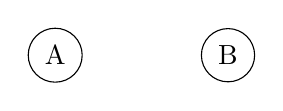
\begin{tikzpicture}[
  node distance=1cm and 1cm,
  mynode/.style={draw,circle,align=center}
]
\node[mynode] (A) {A};
\node[mynode, right=1.5cm of A] (B) {B};
\end{tikzpicture}
\caption{Independence}
\label{ref:independence}
\end{figure}

As seen in Figure~\ref{ref:independence}, $A$ and $B$ are independent:
\begin{definition}
P(A,B) = P(A)P(B)
\end{definition}

\begin{definition}
$P(A\vert B) = P(A)$ or $P(B\vert A) = P(B)$ 
\end{definition}


\subsection{Conditional Independence}

\begin{figure}[h!]
\centering
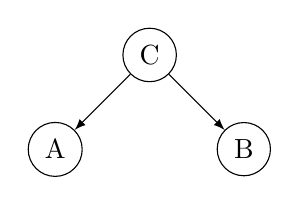
\begin{tikzpicture}[
  node distance=1cm and 0cm,
  mynode/.style={draw,circle,align=center}
]
\node[mynode] (C) {C};
\node[mynode,below left=1cm of C] (A) {A};
\node[mynode,below right=1cm of C] (B) {B};
\path (C) edge[-latex] (A)
(C) edge[-latex] (B);
\end{tikzpicture}
\caption{Conditional independence}
\label{ref:condindependence1}
\end{figure}


As seen in Figure~\ref{ref:condindependence1}, $A$ and $B$ are conditionally independent, given $C$:
\begin{definition}
$P(A,B\vert C) = P(A\vert C)P(B\vert C)$
\end{definition}

\begin{definition}
$P(A\vert B,C) = P(A\vert C)$ and $P(B\vert A,C) = P(B\vert C)$
\end{definition}

$A\independent B \vert C \neq A\independent B$
\\

As seen in Figure~\ref{ref:condindependence2}, $A\independent B$ when $C$ is unknown. When $C$ is known, $A$ and $B$ are dependent. Therefore, independence does not imply conditional independence.


\begin{figure}[h!]
\centering
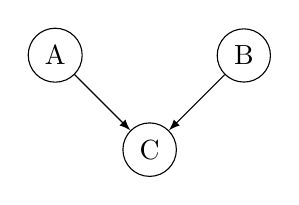
\begin{tikzpicture}[
  node distance=1cm and 1cm,
  mynode/.style={draw,circle,align=center}
]
\node[mynode] (C) {C};
\node[mynode,above left=1cm of C] (A) {A};
\node[mynode,above right=1cm of C] (B) {B};
\path (A) edge[-latex] (C)
(B) edge[-latex] (C);
\end{tikzpicture}
\caption{Conditional independence}
\label{ref:condindependence2}
\end{figure}


\section{Conditional Probabilities} 
\begin{definition}[Complement]
$P(\neg A\vert B) = 1 - P(A\vert B)$
\end{definition}

For $a$ and $b$ to be true, $b$ needs to be true and $a$ needs to be true given $b$:
\begin{definition}[Product rule]
$P(A,B) =P(A\vert B)P(B)$
\end{definition}

\subsection{Total Probability}
\begin{definition}
$P(A) = \sum_{b\in B}{P(A,b)} = \sum_{b\in B}{P(A\vert b)P(b)}$
\end{definition}

\begin{definition}[For conditional variables]
$P(A\vert C) = \sum_{b\in B}{P(A\vert C,b)P(b\vert C)}$
\end{definition}

\subsection{Bayes' Rule}
Applying product rule and total probability:
\begin{definition}
$P(A\vert B) = \frac{P(B\vert A)P(A)}{\sum_{a\in A}{P(B\vert a)P(a)}} = \frac{P(B\vert A)P(A)}{P(B)}$
\end{definition}

The terminology is: $Posterior = \frac{Prior\times Likelihood}{Normalizer}$\\

The normalizer might be difficult to calculate. It can be substituted with pseudo probabilities:
\begin{enumerate}
\item $P'(A\vert B) = P(B\vert A)P(A)$ and $P'(\neg A\vert B) = P(B\vert \neg A)P(\neg A)$
\item $P(A\vert B) = \alpha P'(A\vert B)$ and $P(\neg A\vert B) = \alpha P'(\neg A\vert B)$ with $\alpha = \frac{1}{P'(A\vert B) + P'(\neg A\vert B)}$
\end{enumerate}

\begin{definition}[General Bayes' rule]
$P(A\vert B,e) = \frac{P(B\vert A,e)P(A\vert e)}{P(B\vert e)}$
\end{definition}


\section{Bayes Networks}
Bayes networks define probability distributions over random variables and allow compact specification of full joint distributions. The joint probability of the network shown in Figure~\ref{ref:samplenetwork} is: $P(A,B,C,D,E)=P(A)(B)P(C\vert A,B)P(D\vert C)P(E\vert C)$. The general equation is:
\begin{definition}
$P(x_1,...,x_n) = \prod_{i=1}^{n}{P(x_i\vert parents(X_i))}$
\end{definition}


\begin{figure}[h!]
\centering
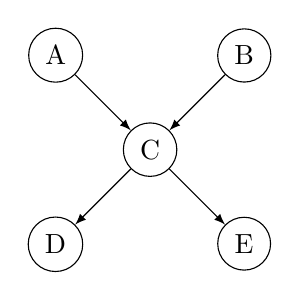
\begin{tikzpicture}[
  node distance=1cm and 1cm,
  mynode/.style={draw,circle,align=center}
]
\node[mynode] (C) {C};
\node[mynode,above left=1cm of C] (A) {A};
\node[mynode,above right=1cm of C] (B) {B};
\node[mynode,below left=1cm of C] (D) {D};
\node[mynode,below right=1cm of C] (E) {E};
\path (A) edge[-latex] (C)
(B) edge[-latex] (C)
(C) edge[-latex] (D)
(C) edge[-latex] (E);
\end{tikzpicture}
\caption{Sample Bayes network}
\label{ref:samplenetwork}
\end{figure}

\subsection{D-Separation}
Stands for direction-dependent separation. D-separated variables are independent. $X$ and $Y$ are d-separated if there is no active path between them. Paths consists of {\bf triplets} as defined in Table~\ref{ref:triplets}. An inactive triplet makes an entire path inactive.

\begin{table}[h!]
\begin{center}
\begin{tabular}{|c|c|}
\hline
Active & Inactive \\
\hline
\hline
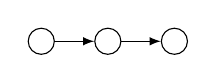
\begin{tikzpicture}[
  node distance=1cm and 1cm,
  mynode/.style={draw,circle,align=center}
]
\node[mynode] (A) {};
\node[mynode, right=0.5cm of A] (B) {};
\node[mynode, right=0.5cm of B] (C) {};
\path (A) edge[-latex] (B)
(B) edge[-latex] (C);
\end{tikzpicture}
Causal chain
&
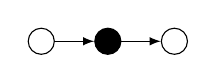
\begin{tikzpicture}[
  node distance=1cm and 1cm,
  mynode/.style={draw,circle,align=center}
]
\node[mynode] (A) {};
\node[mynode, right=0.5cm of A, fill=black] (B) {};
\node[mynode, right=0.5cm of B] (C) {};
\path (A) edge[-latex] (B)
(B) edge[-latex] (C);
\end{tikzpicture}
\\
\hline
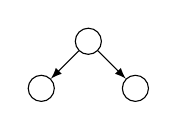
\begin{tikzpicture}[
  node distance=1cm and 1cm,
  mynode/.style={draw,circle,align=center}
]
\node[mynode] (C) {};
\node[mynode,below left=0.5cm of C] (A) {};
\node[mynode,below right=0.5cm of C] (B) {};
\path (C) edge[-latex] (A)
(C) edge[-latex] (B);
\end{tikzpicture}
Common cause
&
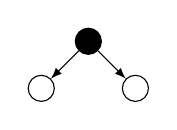
\begin{tikzpicture}[
  node distance=1cm and 1cm,
  mynode/.style={draw,circle,align=center}
]
\node[mynode, fill=black] (C) {};
\node[mynode,below left=0.5cm of C] (A) {};
\node[mynode,below right=0.5cm of C] (B) {};
\path (C) edge[-latex] (A)
(C) edge[-latex] (B);
\end{tikzpicture}
\\
\hline
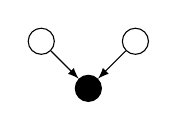
\begin{tikzpicture}[
  node distance=1cm and 1cm,
  mynode/.style={draw,circle,align=center}
]
\node[mynode,fill=black] (C) {};
\node[mynode,above left=0.5cm of C] (A) {};
\node[mynode,above right=0.5cm of C] (B) {};
\path (A) edge[-latex] (C)
(B) edge[-latex] (C);
\end{tikzpicture}
Common effect
&
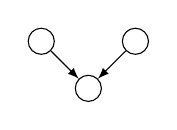
\begin{tikzpicture}[
  node distance=1cm and 1cm,
  mynode/.style={draw,circle,align=center}
]
\node[mynode] (C) {};
\node[mynode,above left=0.5cm of C] (A) {};
\node[mynode,above right=0.5cm of C] (B) {};
\path (A) edge[-latex] (C)
(B) edge[-latex] (C);
\end{tikzpicture}
\\
\hline
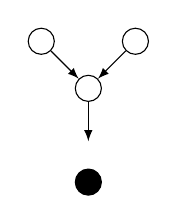
\begin{tikzpicture}[
  node distance=1cm and 1cm,
  mynode/.style={draw,circle,align=center}
]
\node[mynode] (C) {};
\node[mynode,above left=0.5cm of C] (A) {};
\node[mynode,above right=0.5cm of C] (B) {};
\node[mynode,below=0.5cm of C,color=white] (D) {};
\node[mynode,below=0cm of D, fill=black] (E) {};
\path (A) edge[-latex] (C)
(B) edge[-latex] (C)
(C) edge[-latex] (D);
\end{tikzpicture}
&
\\
\hline
\end{tabular}
\end{center}
\caption{Active and inactive triplets with known variables filled}
\label{ref:triplets}
\end{table}


\chapter{General}
\section{Terminology}
\subsection{Intelligent Agents}
An {\bf agent} operates autonomously. A {\bf rational agent} acts to achieve the best outcome or expected outcome if there is uncertainty. An {\bf agent program} implements the {\bf agent function} which maps perceptions to actions.

\subsection{Task Environments}
{\bf Fully observable} vs. {\bf partially observable}: the agent's sensors perceive the complete state of the relevant environment at each point in time. {\bf Deterministic} vs. {\bf stochastic}: the agent's state and action uniquely determine the next state. {\bf Discrete} vs. {\bf continuous}: finite amount of states, actions and outcomes. {\bf Benign} vs. {\bf adversarial}: there is no opponent.


\chapter{Problem Solving}
\section{General Search}

Table~\ref{ref:search} compares general search algorithms.

\begin{table}[h!]
\begin{center}
\begin{tabular}{|l||c|c|c|}
\hline
 & Breadth-first & Uniform-cost & Depth-first\\
\hline
\hline
Expansion order
&
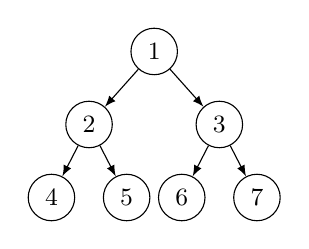
\begin{tikzpicture}[
  node distance=1cm and 1cm,
  mynode/.style={draw,circle,align=center},
  font=\small
]
\node[mynode] (A) {1};
\node[mynode,below left=0.5cm and 0.4 of A] (B) {2};
\node[mynode,below right=0.5cm and 0.4 of A] (C) {3};
\node[mynode,below left=0.5cm and 0.05 of B] (D) {4};
\node[mynode,below right=0.5cm and 0.05 of B] (E) {5};
\node[mynode,below left=0.5cm and 0.05 of C] (F) {6};
\node[mynode,below right=0.5cm and 0.05 of C] (G) {7};
\path (A) edge[-latex] (B)
(A) edge[-latex] (C)
(B) edge[-latex] (D)
(B) edge[-latex] (E)
(C) edge[-latex] (F)
(C) edge[-latex] (G);
\end{tikzpicture}
&
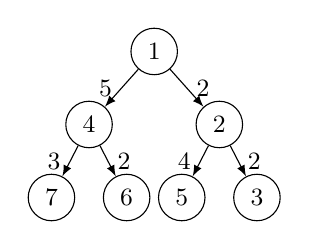
\begin{tikzpicture}[
  node distance=1cm and 1cm,
  mynode/.style={draw,circle,align=center},
  font=\small
]
\node[mynode] (A) {1};
\node[mynode,below left=0.5cm and 0.4 of A] (B) {4};
\node[mynode,below right=0.5cm and 0.4 of A] (C) {2};
\node[mynode,below left=0.5cm and 0.05 of B] (D) {7};
\node[mynode,below right=0.5cm and 0.05 of B] (E) {6};
\node[mynode,below left=0.5cm and 0.05 of C] (F) {5};
\node[mynode,below right=0.5cm and 0.05 of C] (G) {3};
\path (A) edge[-latex] node[left] {5} (B)
(A) edge[-latex] node[right] {2} (C)
(B) edge[-latex] node[left] {3} (D)
(B) edge[-latex] node[right] {2} (E)
(C) edge[-latex] node[left] {4} (F)
(C) edge[-latex] node[right] {2} (G);
\end{tikzpicture}
&
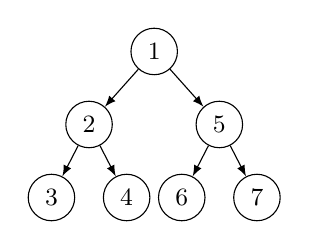
\begin{tikzpicture}[
  node distance=1cm and 1cm,
  mynode/.style={draw,circle,align=center},
  font=\small
]
\node[mynode] (A) {1};
\node[mynode,below left=0.5cm and 0.4 of A] (B) {2};
\node[mynode,below right=0.5cm and 0.4 of A] (C) {5};
\node[mynode,below left=0.5cm and 0.05 of B] (D) {3};
\node[mynode,below right=0.5cm and 0.05 of B] (E) {4};
\node[mynode,below left=0.5cm and 0.05 of C] (F) {6};
\node[mynode,below right=0.5cm and 0.05 of C] (G) {7};
\path (A) edge[-latex] (B)
(A) edge[-latex] (C)
(B) edge[-latex] (D)
(B) edge[-latex] (E)
(C) edge[-latex] (F)
(C) edge[-latex] (G);
\end{tikzpicture}
\\
\hline
Expansion strategy & Shallowest & Cheapest & Deepest\\
\hline
Optimal & Yes & Yes & No\\
\hline
Complete & Yes & Yes & No\\
\hline
Frontier size ($n$ levels) & $2n$ & $2n$ & $n$\\
\hline
\end{tabular}
\end{center}
\caption{Comparison of search algorithms}
\label{ref:search}
\end{table}

\section{A* Search}
$A*$ expands the path with that has the minimum value $f$.

\begin{definition}[A* cost function]
$f = g + h$ with $g(path) =$ current path cost and $h(path) = h(s) =$ estimated distance to goal
\end{definition}

$f$ is a {\bf heuristic function}. $A*$ finds lowest cost path if: $h(s) <$ true cost. Subsequently, $h$ never overestimates and is optimistic/admissible. See Figure~\ref{ref:heuristic} for an example.

\begin{figure}[h!]
\centering
\begin{subfigure}[b]{0.3\textwidth}
\begin{tabular}{|c|c|c|c|c|c|}
\hline
S &\cellcolor{black}&&&& \\
\hline
&\cellcolor{black}&&&& \\
\hline
&\cellcolor{black}&&&& \\
\hline
&\cellcolor{black}&&&& \\
\hline
&&&&&G \\
\hline
\end{tabular}
\end{subfigure}
\begin{subfigure}[b]{0.3\textwidth}
\begin{tabular}{|c|c|c|c|c|c|}
\hline
9&8&7&6&5&4 \\
\hline
8&7&6&5&4&3 \\
\hline
7&6&5&4&3&2 \\
\hline
6&5&4&3&2&1 \\
\hline
5&4&3&2&1&0 \\
\hline
\end{tabular}
\end{subfigure}
\caption{Sample world and heuristic}
\label{ref:heuristic}
\end{figure}


\section{Policy}
A {\bf policy} specifies what an agent should do for any state that the agent might reach. An {\bf optimal policy} is a policy that yields the highest expected {\bf utility} (meaning "the quality of being useful"). See Figure~\ref{ref:policy} for an example.

\begin{figure}[h!]
\centering
\begin{subfigure}[b]{0.3\textwidth}
\begin{tabular}{|c|c|c|c|c|c|}
\hline
&\cellcolor{black}&&&& \\
\hline
&\cellcolor{black}&&&& \\
\hline
&\cellcolor{black}&&&& \\
\hline
&\cellcolor{black}&&&& \\
\hline
&&&&\cellcolor{black}&G \\
\hline
\end{tabular}
\end{subfigure}
\begin{subfigure}[b]{0.3\textwidth}
\begin{tabular}{|c|c|c|c|c|c|}
\hline
$\downarrow$&&$\rightarrow$&$\rightarrow$&$\rightarrow$&$\downarrow$ \\
\hline
$\downarrow$&&$\rightarrow$&$\rightarrow$&$\rightarrow$&$\downarrow$ \\
\hline
$\downarrow$&&$\rightarrow$&$\rightarrow$&$\rightarrow$&$\downarrow$ \\
\hline
$\downarrow$&&$\rightarrow$&$\rightarrow$&$\rightarrow$&$\downarrow$ \\
\hline
$\rightarrow$&$\rightarrow$&$\uparrow$&$\uparrow$&&* \\
\hline
\end{tabular}
\end{subfigure}
\caption{Sample world and policy}
\label{ref:policy}
\end{figure}


\end{document}